\documentclass[11pt]{article}
\usepackage{geometry,graphicx}
\usepackage{tikz}
\usetikzlibrary{arrows,calc}
\geometry{
  lmargin = 1in,
  rmargin = 1in,
  tmargin = 1in,
  bmargin = 1in
}

\begin{document}
\title{Variations on the Hamiltonian Cycle Problem}
\author{Karthik Gopalan}
\maketitle

\vfill
\section{Abstract}
The Hamiltonian Cycle Problem is easily stated as: given a graph G,
with verticies V and edges E, find a \emph{cycle} that visits every vertex.
Everyone has heard that it is NP-Complete but most people have not seen the proof.
This paper will enlighten those people by providing detailed proofs of why 4 classic variations of
the problem are NP-Complete.

\section{Introdution}
The Hamiltonian Cycle Problem is easily stated as: given a graph G, 
with verticies V and edges E, find a \emph{cycle} that visits every vertex. 
A natural variation would be given a graph G, find a \emph{path} that starts at some 
vertex $s \in V$, visits each vertex exactly once, and ends at vertex $t \in V$. Other problems can be synthesized
by varying the graph G. This paper will focus on proving that the following variations are NP-Complete

\begin{enumerate}
\item \{G $|$ G is a directed graph with a directed Ham Cycle\}
\item \{G $|$ G is a directed graph with a directed Ham Path\}
\item \{G $|$ G is an undirected graph with an undirected Ham Cycle\}
\item \{G $|$ G is an undirected graph with an undirected Ham Path\}
\end{enumerate}

To prove that all of these problems are NP-Complete, we first show that 3-SAT, a known
NP-complete problem, is polynomial time reducible to problem 2. Then we show that problem
2 is polynomial time reducible to problems 1 and 4, and finally that problem 4 is poly
time reducible to problem 3.

\newpage
Here is a flowchart of the proof:
\begin{figure}[h]
\centering
\includegraphics[width=.5\textwidth]{ProofOutline.png}
\end{figure}

All of the credit for my understanding of these proofs goes to Michael Sipster and his book, \emph{Introduction
to the Theory of Computation}.

\section{3-SAT $\leq_{P}$ Directed Ham Path}
The Hamiltonian Path problem is in NP because a solution to the problem can be verified 
in polynomial time with a certificate. The certificate is the path represented by an 
ordering of nodes. To verify a Hamiltonian path; make sure each node is in the path once, and for each consecutive pair of nodes in the list verify that an edge exists between
them. This can obviously be done in polynomial time.

The boolean satisfiability problem (SAT) is: given a boolean formula $\phi$ with $n$
variables seperated by $\land$'s $\lor$'s and $\neg$'s, find an assignment of the 
variables such that $\phi = 1$. 3-SAT is an instance of SAT where the formula is in conjunctive normal form
with clauses of size 3. 3-SAT is NP-Complete.

Given a 3cnf-formula $\phi$ with $k$ clauses, n variables $x_{1} \cdots x_{n}$, and 
literals $x_{i}$, $\overline{x_{i}}$ represented by $a$, $b$, or $c$.

$$
\phi = (a_{1} \lor b_{1} \lor c_{1}) \land (a_{2} \lor b_{2} \lor c_{2}) 
\land \cdots \land (a_{k} \lor b_{k} \lor c_{k})
$$

We must turn $\phi$ into a directed graph G that holds the 
property that a Hamiltonian Path between verticies s and t exists if and only if $\phi$ has a 
satisfing assignment. To start, we must represent each variable $x_{i}$ with a gadget that
contains a horizontal row of $3k + 1$ nodes, a node with edges to each end of the row, and
a node with incoming edges from each end of the row. The structure looks like this:

\begin{center}
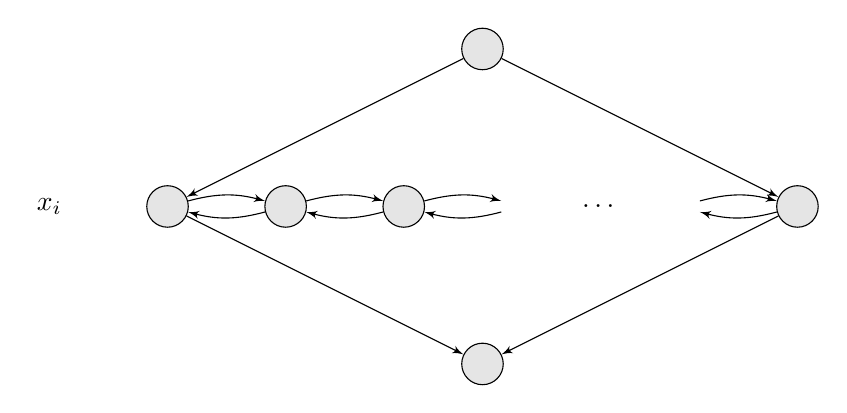
\begin{tikzpicture}
\tikzset{vertex/.style = {shape=circle,draw,minimum size=1.5em, fill=gray!20}}
\tikzset{edge/.style = {->,> = latex'}}
% vertices
\node[] (lab) at (-1.5,0) {$x_{i}$};
\node[vertex] (a) at  (0,0) {};
\node[vertex] (b) at  (4,2) {};
\node[vertex] (c) at  (8,0) {};
\node[vertex] (d) at  (4,-2) {};
\node[vertex] (a1) at (1.5,0) {};
\node[vertex] (a2) at (3,0) {};
%edges
\draw[edge] (b) to (a);
\draw[edge] (b) to (c);
\draw[edge] (a) to (d);
\draw[edge] (c) to (d);

\draw[edge] (a)  to[bend left=15] (a1);
\draw[edge] (a1) to[bend left=15] (a);

\draw[edge] (a1) to[bend left=15] (a2);
\draw[edge] (a2) to[bend left=15] (a1);

\path (a2) to node {\dots} (c);
\node [shape=circle,minimum size=1.5em] (a3) at (4.5,0) {};
\draw[edge] (a2) to[bend left=15] (a3);
\draw[edge] (a3) to[bend left=15] (a2);

\node [shape=circle,minimum size=1.5em] (c1) at (6.5,0) {};
\draw[edge] (c) to[bend left=15] (c1);
\draw[edge] (c1) to[bend left=15] (c);
\end{tikzpicture}
\end{center}

\newpage
Every clause is represented as a single node like so:
\begin{center}
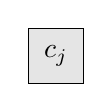
\begin{tikzpicture}
\tikzset{vertex/.style = {shape=rectangle,draw,minimum size=2em, fill=gray!20}}
\node[vertex] (cj) at (1.5,0) {$c_{j}$};
\end{tikzpicture}
\end{center}

When all of the variables are connected the graph will look like:

\begin{center}
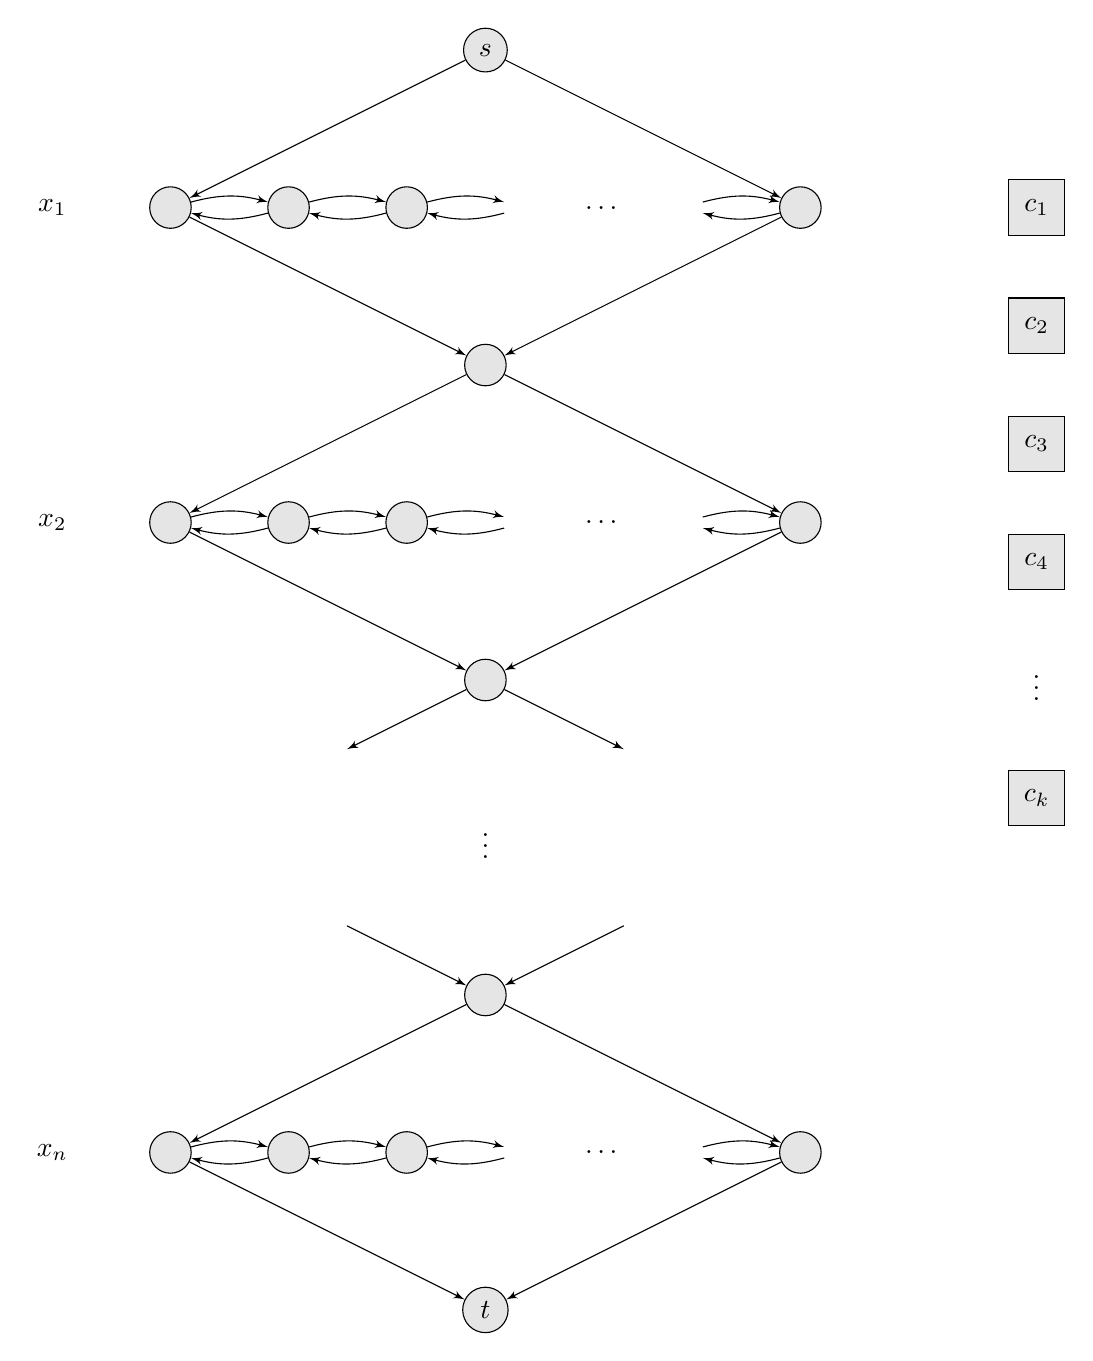
\begin{tikzpicture}
\tikzset{vertex/.style = {shape=circle,draw,minimum size=1.5em, fill=gray!20}}
\tikzset{clause/.style = {shape=rectangle,draw,minimum size=2em, fill=gray!20}}
\tikzset{edge/.style = {->,> = latex'}}
%vertices
% ----- x1
\node[] (lab) at (-1.5,0) {$x_{1}$};
\node[vertex] (a) at  (0,0) {};
\node[vertex] (b) at  (4,2) {$s$};
\node[vertex] (c) at  (8,0) {};
\node[vertex] (d) at  (4,-2) {};
\node[vertex] (a1) at (1.5,0) {};
\node[vertex] (a2) at (3,0) {};

% ---- x2
\node[] (lab) at (-1.5,-4) {$x_{2}$};
\node[vertex] (a_2) at  (0,-4) {};
\node[vertex] (c_2) at  (8,-4) {};
\node[vertex] (d_2) at  (4,-6) {};
\node[vertex] (a1_2) at (1.5,-4) {};
\node[vertex] (a2_2) at (3,-4) {};


%edges
\draw[edge] (b) to (a);
\draw[edge] (b) to (c);
\draw[edge] (a) to (d);
\draw[edge] (c) to (d);

\draw[edge] (a)  to[bend left=15] (a1);
\draw[edge] (a1) to[bend left=15] (a);

\draw[edge] (a1) to[bend left=15] (a2);
\draw[edge] (a2) to[bend left=15] (a1);

\path (a2) to node {\dots} (c);
\node [shape=circle,minimum size=1.5em] (a3) at (4.5,0) {};
\draw[edge] (a2) to[bend left=15] (a3);
\draw[edge] (a3) to[bend left=15] (a2);

\node [shape=circle,minimum size=1.5em] (c1) at (6.5,0) {};
\draw[edge] (c) to[bend left=15] (c1);
\draw[edge] (c1) to[bend left=15] (c);

%---- x2
\draw[edge] (d) to (a_2);
\draw[edge] (d) to (c_2);
\draw[edge] (a_2) to (d_2);
\draw[edge] (c_2) to (d_2);

\draw[edge] (a_2)  to[bend left=15] (a1_2);
\draw[edge] (a1_2) to[bend left=15] (a_2);

\draw[edge] (a1_2) to[bend left=15] (a2_2);
\draw[edge] (a2_2) to[bend left=15] (a1_2);

\path (a2_2) to node {\dots} (c_2);
\node [shape=circle,minimum size=1.5em] (a3_2) at (4.5,-4) {};
\draw[edge] (a2_2) to[bend left=15] (a3_2);
\draw[edge] (a3_2) to[bend left=15] (a2_2);

\node [shape=circle,minimum size=1.5em] (c1_2) at (6.5,-4) {};
\draw[edge] (c_2) to[bend left=15] (c1_2);
\draw[edge] (c1_2) to[bend left=15] (c_2);

\node [shape=circle,minimum size=1.5em] (d_inv1) at (2,-7) {};
\node [shape=circle,minimum size=1.5em] (d_inv2) at (6,-7) {};
\draw[edge] (d_2) to (d_inv1);
\draw[edge] (d_2) to (d_inv2);
%---- xn

\node[] (lab) at (-1.5,-12) {$x_{n}$};
\node[vertex] (a_n) at  (0,-12) {};
\node[vertex] (b_n) at  (4,-10) {};
\node[vertex] (c_n) at  (8,-12) {};
\node[vertex] (d_n) at  (4,-14) {$t$};
\node[vertex] (a1_n) at (1.5,-12) {};
\node[vertex] (a2_n) at (3,-12) {};
\node [shape=circle,minimum size=1.5em] (d_inv) at (2,-9) {};
\node [shape=circle,minimum size=1.5em] (d_invn) at (6,-9) {};

%-----clauses
\node[clause] (cl1) at (11,0) {$c_{1}$};
\node[clause] (cl2) at (11,-1.5) {$c_{2}$};
\node[clause] (cl3) at (11,-3) {$c_{3}$};
\node[clause] (cl4) at (11,-4.5) {$c_{4}$};
\node[clause] (cl5) at (11,-7.5) {$c_{k}$};

\path (cl4) to node {$\vdots$} (cl5);

%---
\draw[edge] (d_inv) to (b_n);
\draw[edge] (d_invn) to (b_n);

\draw[edge] (a_n)  to[bend left=15] (a1_n);
\draw[edge] (a1_n) to[bend left=15] (a_n);

\draw[edge] (a1_n) to[bend left=15] (a2_n);
\draw[edge] (a2_n) to[bend left=15] (a1_n);

\path (a2_n) to node {\dots} (c_n);
\node [shape=circle,minimum size=1.5em] (a3_n) at (4.5,-12) {};
\draw[edge] (a2_n) to[bend left=15] (a3_n);
\draw[edge] (a3_n) to[bend left=15] (a2_n);

\node [shape=circle,minimum size=1.5em] (c1_n) at (6.5,-12) {};
\draw[edge] (c_n) to[bend left=15] (c1_n);
\draw[edge] (c1_n) to[bend left=15] (c_n);


\path (d_2) to node {$\vdots$} (b_n);

\draw[edge] (b_n) to (a_n);
\draw[edge] (b_n) to (c_n);
\draw[edge] (a_n) to (d_n);
\draw[edge] (c_n) to (d_n);
\end{tikzpicture}
\end{center}

\newpage

All that is left is to insert the edges connecting the clauses. 
If the literal $x_{i}$ appears in clause $c_{j}$ we will go to the horizontal row of $x_{i}$. 
Then add an edge from the $3j^{th}$ node to node $c_{j}$ and an edge from node $c_{j}$
to the $3j+1^{th}$ node. 
If the literal $\overline{x_{i}}$ appears in clause $c_{j}$ we will go to the horizontal row of $x_{i}$.
Then add an edge from the $3j+1^{th}$ node to node $c_{j}$ and an edge from node $c_{j}$
to the $3j^{th}$ node. The first case is illustrated below.

\begin{center}
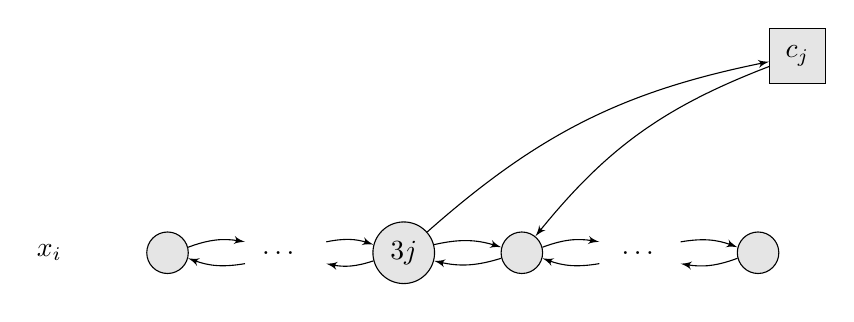
\begin{tikzpicture}
\tikzset{vertex/.style = {shape=circle,draw,minimum size=1.5em, fill=gray!20}}
\tikzset{clause/.style = {shape=rectangle,draw,minimum size=2em, fill=gray!20}}
\tikzset{edge/.style = {->,> = latex'}}
\node[] (lab) at (-1.5,0) {$x_{i}$};
\node[vertex] (1) at (0,0) {};
\node[vertex] (2) at (3,0) {$3j$};
\node[vertex] (3) at (4.5,0) {};
\node[vertex] (4) at (7.5,0) {};
\node[shape=circle,minimum size=3em] (l) at (1.5,0) {};
\node[shape=circle,minimum size=3em] (r) at (6,0) {};

\draw[edge] (1) to [bend left=15] (l);
\draw[edge] (l) to [bend left=15] (2);
\draw[edge] (2) to [bend left=15] (3);
\draw[edge] (3) to [bend left=15] (r);
\draw[edge] (4) to [bend left=15] (r);
\draw[edge] (r) to [bend left=15] (4);
\draw[edge] (r) to [bend left=15] (3);
\draw[edge] (3) to [bend left=15] (2);
\draw[edge] (2) to [bend left=15] (l);
\draw[edge] (l) to [bend left=15] (1);

\path (1) to node {\dots} (2);
\path (3) to node {\dots} (4);

\node[clause] (cj) at (8,2.5) {$c_{j}$};
\draw[edge] (2) to [bend left=15, near start] (cj);
\draw[edge] (cj) to [bend right=15, near start] (3);

\end{tikzpicture}
\end{center}

Now that the clauses are connected, the graph is complete but how do we know it works?

\subsection{Proof}
There are only two ways for a path to touch every node in each diamond shaped gadget. 
\begin{enumerate} 
\item {Start at the top, follow the left edge, traverse the horizontal row to
the \emph{right}, and finally take the edge to the bottom node.}
\item {Start at the top,
 follow the right edge, traverse the horizontal row to the \emph{left}, and take the 
edge to the bottom node.}
\end{enumerate}
Now assume that $\phi$ is satisfiable. If $x_{i}$ is set to true, follow path 1 through 
the appropriate diamond. If $x_{i}$ is set to false, follow path 2. In order to complete the path, we must connect the clause nodes.
For each clause, pick a literal that was assigned true. If we pick $x_{i}$ in clause
$c_{j}$ redirect our path from the $3j^{th}$ node to the clause node and back to the $3j
+1^{th}$ node. If $\overline{x_{i}}$ is assigned true in clause $c_{j}$, then $x_{i}$ is
 false and we are following path 2 through the diamond. Therefore, the path is going the
right direction to allow a detour from the $3j+1^{th}$ node to the clause node and a return to the $3j^{th}$ node. Now
 that the clause nodes are included, the Hamiltonian Path is complete.

To finish the proof we must show that if G has a Hamiltonian Path, $\phi$ has a satisfying assignment.
In order for the satisfying assignment to be read from the graph, every horizontal row
of nodes must be traversed from left to right or right to left. If they are mixed, the
variable's assignment will be unclear. The only way to get a mixed assignment is if
a path enters a clause from one diamond and then follows an edge to another. 
If we eventually got back to the original diamond, the only way to visit every node in
the row is to traverse the opposite way. Therefore, the path will be stuck inside of a 
diamond and will not be able to touch every vertex. So any Hamiltonian Path must start
at the top of the structure, traverse each horizontal row in one direction, and end
at the bottom. This path guaruntees a satisfying assignment of $\phi$. Finally, the 
reduction takes time $O(|n(3k+1) + k|)$ which is polynomial.

\section{Directed Ham Path $\leq_{P}$ Undirected Ham Path}
To show that the Undirected Hamiltonian Path problem is NP-Complete, we will show a 
polynomial time reduction from the directed version of the problem. 

Start with a directed graph G with a Hamiltonian Path from $s$ to $t$ and construct an
undirected graph G' with a Hamiltonian Path from $s^{out}$ to $t^{in}$. In order to simulate a 
directed graph, we will replace each node $u \in E - {s,t}$ with three nodes; $u^{in}$, 
$u^{mid}$, and $u^{out}$. For each triplet, add edges connecting $u^{in}$ and $u^{out}$ 
to $u^{mid}$. Finally, add an edge from $a^{out}$ to $b^{in}$ if there exists an edge 
from $a$ to $b$ in G. This tranformation is illustrated below.

\begin{center}
\begin{tabular}{p{3.5in}p{3.5in}}
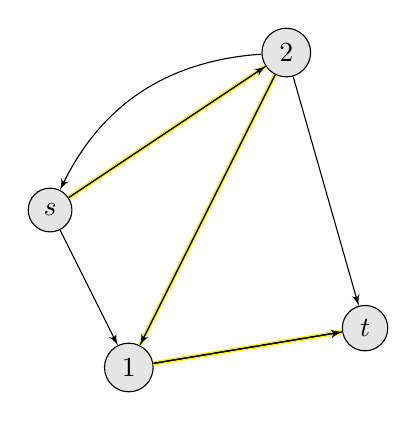
\begin{tikzpicture}
\centering
\tikzset{vertex/.style = {shape=circle,draw,minimum size=1.5em, fill=gray!20}}
\tikzset{edge/.style = {->,> = latex'}}
\foreach \pos/\name in {{(0,0)/s}, {(1,-2)/1}, {(3,2)/2}, {(4,-1.5)/t}}
\node[vertex] (\name) at \pos {$\name$}; 

\foreach \from/\to in {s/2,2/1,1/t}{
\draw[preaction={%But before that
draw,yellow,-,% Draw yellow without any arrow head
double=yellow,
double distance=2\pgflinewidth,
}] (\from) to (\to);
}


\foreach \from/\to in {s/1, 1/t, 2/1, 1/t, 2/t, s/2}
\draw [edge] (\from) to (\to);

\draw[edge] (2) to [bend right] (s);
\end{tikzpicture}

&
\centering
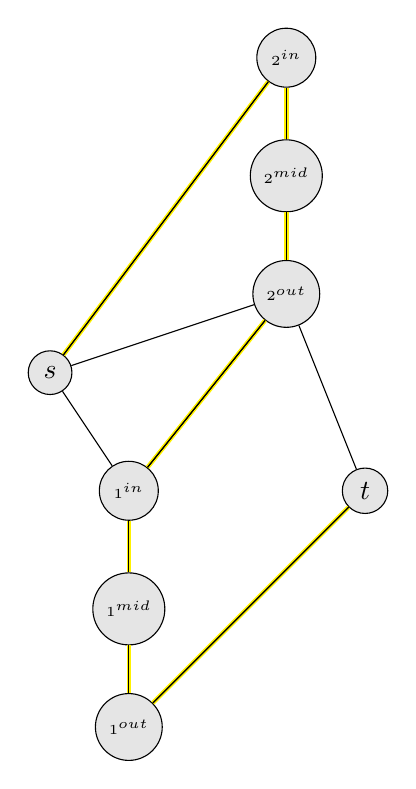
\begin{tikzpicture}
\tikzset{vertex/.style = {shape=circle,draw,minimum size=1.5em, fill=gray!20}}
\tikzset{edge/.style = {- = latex'}}

\node[vertex] (s) at (0,0) {$s$};
\node[vertex] (t) at (4,-1.5) {$t$};

\foreach \pos/\name in {{(1,-1.5)/1^{in}}, {(1,-3)/1^{mid}}, {(1,-4.5)/1^{out}}, {(3,4)/2^{in}}, {(3,2.5)/2^{mid}}, {(3,1)/2^{out}}}
\node[vertex] (\name) at \pos {\tiny $\name$};

\foreach \from/\to in {1^{in}/1^{mid}, 1^{mid}/1^{out}, 2^{in}/2^{mid}, 2^{mid}/2^{out}, 1^{out}/t, s/2^{in}, 2^{out}/1^{in}}{
\draw[preaction={%But before that                                                
draw,yellow,-,% Draw yellow without any arrow head                                        
double=yellow,
double distance=2\pgflinewidth,
}] (\from) to (\to);
}

\foreach \from/\to in {1^{in}/1^{mid}, 1^{mid}/1^{out}, 2^{in}/2^{mid}, 2^{mid}/2^{out}, s/1^{in}, 1^{out}/t, 2^{out}/1^{in}, 2^{out}/t, s/2^{in}, 2^{out}/s}
\draw [edge] (\from) to (\to);

\end{tikzpicture}
\end{tabular}
\end{center}

I claim that G has a Hamiltonian Path from $s$ to $t$ if and only if G' has a Hamiltonian Path from $s'$ to $t'$.
To prove the left to right implication, imagine a Hamiltonian path starts at $s$, 
passes through some ordering of $u_{i}$'s, and finally ends at $t$. Like so:
$$s \rightarrow u_{1} \rightarrow u_{2} \rightarrow u_{3} \rightarrow \dots \rightarrow u_{|E|-2} \rightarrow t$$
Since our construction just replaces nodes by triplets of nodes, the same path in G' would look 
like:
$$s_{out} \rightarrow u_{1}^{in} \rightarrow u_{1}^{mid} \rightarrow u_{1}^{out} \rightarrow u_{2}^{in} \rightarrow u_{2}^{mid} \rightarrow 
u_{2}^{out} \rightarrow \dots \rightarrow t^{in}$$

To prove the right to left implication, I will describe the Hamiltonian Path in G'. 
Start at $s^{out}$ and follow an edge to some $u_i^{in}$. We have to go to $u_i^{mid}$ 
because there is no other way to incorporate it in the path. The next node has to be
$u_i^{out}$ and from there we can take an edge to $u_j^{in}$ and traverse another triplet.
 If you repeat this procedure until you reach $t^{in}$ you will derive a path that 
resembles the one above. Since paths of this form have a directed equivalent, the proof is
complete. This reduction takes time $O(2|V| + 2|E|)$ since you need to add two verticies
and two nodes in G' for almost every node in G.

\section{Dir Ham Path $\leq_P$ Dir Ham Cycle \textbf{AND} \\ Undir Ham Path $\leq_P$ Undir Ham}
I know what you are thinking: ``Karthik how are you going to show two poly time reductions
in one section!??'' I'll show you.

Given a graph $G = (V,E)$ (directed or undirected) with a Hamiltonian Path from $s$ to $t$ , I will construct
 the graph $G' = (V,E \cup {(t,s)})$ by just adding an edge from $t$ to $s$. Here is an
illustration of this construction on a simple directed graph.

\begin{center}
\begin{tabular}{p{3.5in}p{3.5in}}
\begin{center}
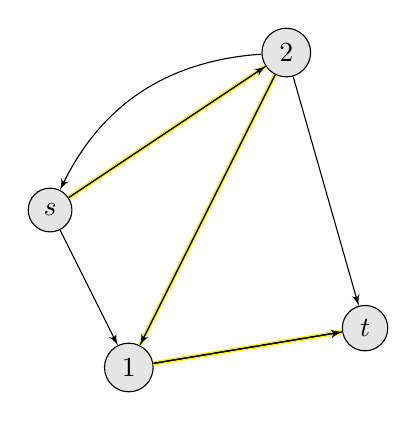
\begin{tikzpicture}

\tikzset{vertex/.style = {shape=circle,draw,minimum size=1.5em, fill=gray!20}}
\tikzset{edge/.style = {->,> = latex'}}
\foreach \pos/\name in {{(0,0)/s}, {(1,-2)/1}, {(3,2)/2}, {(4,-1.5)/t}}
\node[vertex] (\name) at \pos {$\name$};

\foreach \from/\to in {s/2,2/1,1/t}{
\draw[preaction={%But before that
draw,yellow,-,% Draw yellow without any arrow head
double=yellow,
double distance=2\pgflinewidth,
}] (\from) to (\to);
}


\foreach \from/\to in {s/1, 1/t, 2/1, 1/t, 2/t, s/2}
\draw [edge] (\from) to (\to);

\draw[edge] (2) to [bend right] (s);
\end{tikzpicture}
\end{center}
&
\begin{center}
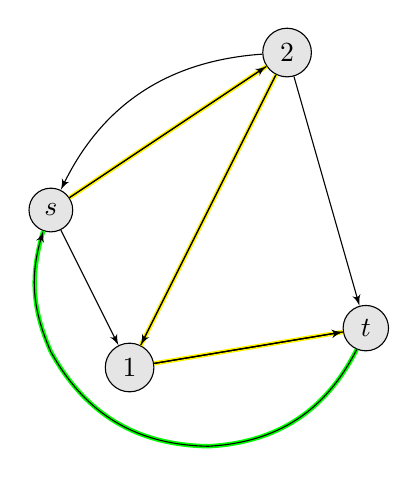
\begin{tikzpicture}

\tikzset{vertex/.style = {shape=circle,draw,minimum size=1.5em, fill=gray!20}}
\tikzset{edge/.style = {->,> = latex'}}
\foreach \pos/\name in {{(0,0)/s}, {(1,-2)/1}, {(3,2)/2}, {(4,-1.5)/t}}
\node[vertex] (\name) at \pos {$\name$};

\foreach \from/\to in {s/2,2/1,1/t}{
\draw[preaction={%But before that
draw,yellow,-,% Draw yellow without any arrow head
double=yellow,
double distance=2\pgflinewidth,
}] (\from) to (\to);
}

\draw[- = latex',
preaction={%But before that
draw,green,-,% Draw yellow without any arrow head
double=green,
double distance=2\pgflinewidth,
}] (t)  to [bend left] (2,-3) to [bend left] (0,-1.8);

\draw[->,> = latex',
preaction={%But before that
draw,green,-,% Draw yellow without any arrow head
double=green,
double distance=2\pgflinewidth,
}] (0,-1.8)  to [bend left=20] (s);


\foreach \from/\to in {s/1, 1/t, 2/1, 1/t, 2/t, s/2}
\draw [edge] (\from) to (\to);

\draw[edge] (2) to [bend right] (s);
\end{tikzpicture}
\end{center}
\end{tabular}
\end{center}
 I claim 
that G has a Hamiltonian Path from $s$ to $t$ if and only if G' has a Hamiltonian 
Cycle. Lets say G has a Hamiltonian Path, if you follow the path from $s$ to $t$ in G'
then take the edge from $t$ to $s$ you will arrive back at $s$, thus completeing the 
cycle. If G' has a Hamiltonian Cycle; start at $s$, follow the cycle to $t$, and then 
stop. This is your Hamiltonian Path. 

This procedure takes constant time with respect to the size of the input.

\end{document}
